\Chapter{A nyelv definíciója}

\section{Általános szempontok}

A saját nyelv kialakításánál az elsődleges szempont a könnyű kezelhetőség volt, hogy bár több nyelvre, több platformra kerülhet lefordításra a kód, a felhasználó, programozó egyszerűen, könnyen tudja megírni a kódot a definiált nyelven, így nem kell minden célnyelvi szintaktikai és szemantikai szabállyal tisztába lennie, azokat külön-külön alkalmaznia.

Ezek alapján a nyelv a Python nyelvhez hasonló megoldásokat és jegyeket hordoz magán, a nyelvi szintaktika és szemantika megvalósításának tekintetében.

Ahhoz, hogy a nyelvet definiálni lehessen az alábbiakban áttekintjük a feladat során célnyelvként tekintett nyelveket általánosan, azok megvalósítását, tulajdonságait, fő elemeit. Majd ezután a saját definiált nyelv tervezett nyelvi elemeit vesszük sorra.

\section{A célnyelvek áttekintése}

A dolgozat szempontjából célnyelvnek azon magasszintű programozási nyelveket tekintjük, melyekre a felhasználó által, a definiált nyelven írt kód a program futtatásának végén lefordul. A program jelenleg nem minden magasszintű programozási nyelvre képes fordítani, tehát nem minden magasszintű programozási nyelv tekinthető célnyelvnek, valamint jelenleg a célnyelvként tekintett magasszintű nyelvek nem minden nyelvi elemét támogatja a program. Ezek a program egy későbbi fejlesztése során elérhetővé válhatnak. Az alábbiakban a dolgozat szempontjából tekintett célnyelveket vizsgáljuk meg röviden.

\subsection{C}

A C nyelv magasszintű, általános célú programozási nyelv, mely az egyik legelterjedtebb programozási nyelv, a ma fellehető számítógép architektúrák szinte mindegyikére készült C fordító. A nyelv sturkturált és szabványos programozási nyelv, ugyanúgy megtalálhatóak itt a vezérlési szerkezetek mint a többi magas szintű nyelvben. Változó deklarálásakor meg kell adni a változó nevét és típusát is, mivel a nyelv erősen típusok nyelv. A változó neve konvenció alapján betűvel kezdődik és utána betűket és számokat tartalmazhat. Ezután egyenlőségjellel adhatjuk meg a változó értékét. C nyelven az utasításokat a sor végén ;-vel zárjuk le. Mivel az egyes utasítások lezárását ; jelzi, a nyelven a sortörések kihagyhatók, ezek a fehér karakterek csak az olvashatóságot növelik, a fordítás során eltávolítására kerülnek. C nyelven írt programok során is az utasítások szekvenciálisan futnak le.

A nyelv nem objektum orientált nyelv, azaz osztályok definíció szintjén nincsenek a nyelvben. Jelen dolgozat további nyelveiben megjelenik ez a funkció, osztályba szervezhető a kód, csakúgy mint a definiált nyelvben is, így valamivel nehezebb C módra történő fordítás. C nyelven a struktúrák találhatók meg, melyek a typedef struct kulcsszóval vezethetnek be. Ebben adhatók meg az osztályokhoz hasonló programelemek. Szintén fontos különbség, hogy a C nyelven megjelennek a pointerek, melyek egy adott változó címere mutató változók. Ezáltal érték szerint és cím szerint is át lehet adni változókat.

C nyelven emellett használható a szelekció, azaz az elágazás. Ezt az if kulcsszó vezeti be, ami után ( és ) között kell megadni az elágazás feltétet. Itt a rendszer azt vizsgálja a megadott feltételek igaz vagy hamis, és aszerint fut le az adott ágban megírt kód. A szelekció többi ágat az else if (feltétel) és az else kulcsszó vezeti be. A C nyelv is ismerni a switch szelekciót, itt is meg kell adni egy kifejezést, változott és a switch belül megadni azon kifejezéseket melyekre az illeszkedést a program vizsgálni fogja.

Emellett a programban megadható iteráció is. Ciklusból a nyelven 3 különböző van, a while, for és do while. Ezek mindegyikéhez kell egy ciklusváltozó, egy feltétel, melyet minden egy ciklusban ellenőriz a rendszer. A for és a while elöl tesztelő ciklus, míg a do while hátul tesztelő, azaz az egyszer biztos le fog futni a cilkusmag, míg az előző kettőben nem biztos. A C nyelvben nincs külön hibakezelés, minden ilyen feladatot a programozónak kell feltételvizsgálattal megoldania, illetve klasszikus esetben nincs automatikus szemétgyűjtő algoritmus sem, a memória felszabadításáról is a programozónak kell gondoskodnia.

\subsection{JavaScript}

A JavaScript egy scriptnyelv, mely leggyakrabban a böngészőben jelenik meg, és kliens oldalon is látható a kódja. A nyelv először MochaScript néven lett létrehozva, majd később a szintaxisa a Java nyelvhez lett hasonló, itt lett a neve JavaScript.

A nyelvet a böngészőkben használt html nyelv statikusságának megtörésére használták, illetve JavaScript segítségével egyszerűen elvégezhető előzetes ellenőrzés az adatokra, mely mellett azonban természetesen mindenképpen kell szerver oldali ellenőrzés is, mivel ahogyan fentebb említettem a JavaScript kód látható böngészőben is különféle eszközökkel, így akár manipulálható is. A kódot a html kódba is ágyazhatjuk, de legtöbbször egy külön .js fáljban van elhelyezve. A JavaScript gyengén típusos nyelv, a változók definiálásakor nem kell típust megjelölni. A változó értéke fogja megadni a változó típusát.

A JavaScriptben is megtalálhatók az ismert vezérlési szerkezetek, ugyanúgy használható az értékadás, szekvencia, szelekció és iteráció is. Sőt még objektum orientálttá is tehető a nyelv. A JavaScriptben külön kifejezéssel lehet változót deklarálni, ez a var kulcsszó, melyet mindig meg kell adni, ezután következik a változó név majd az érték.

Külön meg kell említeni a láthatóságot a JavaScript esetében. Itt a változók alapértelmezetten csak az adott scope-ban elérhetők, ahol létre lettek hozva. Általános esetben mindenképpen egy függvény kerül megírásra, és ebben történik a változók létrehozása, a műveletek elvégzése. A változók csak az adott függvényen belül láthatók ahol létre lettek hozva. Megadhatók azonban olyan módon is a változók, hogy máshonnan is elérhető legyenek, ekkor a függvényen kívül kell deklarálni őket, így globális változókká válnak és elérhetők. Másik módszer ha olyan változóknak adunk értéket amik még nincsenek is deklarálva. A JavaScript ebben az esetben létrehozza a változót, mely azonban globális változóként kerül létrehozásra.

Fentebb említettem a JavaScriptet, mint objektum orientálttá tehető nyelvet. A JavaScriptben általánosságban mindig egy függvényt írunk a function kulcsszóval, még akkor is, ha ez esetleg rejtetten, mondjuk egy jQuery fájlban az alábbi módon nézne ki:

\begin{cpp}
$("data").click(function() {
	utasitasok;
});
\end{cpp}
% $

Látható a fentebbi kódban is megjelenik a function kulcsszó. A nyelv objetum orientáltsága mindössze annyit jelent, hogy egy osztályként használt függvényt írunk meg, majd ennek adunk adattagokat és további függvényeket is, és végül ezt fogjuk használni objektumként, azaz osztályként.

A JavaScript esetében minden utasítássort \texttt{;}-vel kell lezárni szintaktikailag, tehát ebben hasonlít az általánosan vizsgált programozási nyelvekhez.

\subsection{Python}

A Pyhton egy objektum orientált programozási nyelv, mely egyre nagyobb teret hódít egyszerű kezelhetősége és rugalmassága miatt. Guido van Rossum a nyelv megalkotásakor a fent emlíett egyszerűséget tartotta a legfontosabbnak.

A nyelv gyengén típusos nyelv, tehát itt sem kell megadni típusmegjelölést, illetve fontos különbség a többi nyelvhez képest, hogy nem használnak \texttt{;}-t az utasítások lezárásakor, így az utasítások végét a sor vége jelenti. Más magas szintű nyelvekkel ellentétben itt ezért nem is lehetne az egész kódot egy sorban megadni.

Emellett szintén fontos különbség a blokkokat jelző \texttt{\{} és \texttt{\}} hiánya, a nyelv az olvashatóságot is segítendő, a tabulátorokkal történő behúzással jelzi az egyes blokkokat.

Általánosságban egy adott metódus, osztálydefiníció, elágazás, megírásakor a sor végére \texttt{:}-ot teszünk, ezután a következő sortól tabulátor behízással történik az adott feltétel vagy osztály magjának leírása.

A nyelv támogatja az objektum orientált leírást, a class kulcsszóval bevezetett osztályokat lehet megírni, melyben definiálhatunk változókat, metódusokat majd példányosíthatjuk csak úgy mint az általánosságban vizsgált programozási nyelvek esetében.

\subsection{PHP}

A PHP egy szerveroldali nyelv, tulajdonképpen scriptnyelv, az így megírt fájlok futtatásához a fizikai szervergépre valamilyen PHP fordítót kell telepíteni és konfigurálni. Legelterjedtebb manapság még mindig az Apache webszerver, mely a UNIX rendszerekre telepíthető.

Érdemes kiemelni a PHP hiba, illetve figyelmeztetés kijelzését is, mely szerver oldalon, az Apache konfigurációs fáljában, illetve a PHP fájlban is letiltható, illetve engedélyezhető. Érdemes ezt mindig engedélyezni a fejlesztés során, mivel egyéb esetben egyes hibák elfedésre kerülnek a PHP rugalmassága miatt, így a végső eredmény is hibás lehet. Például az alábbi kódban:

\begin{cpp}
<?php
   function multiply ($value) {
      $value = $value * 10;
      return $value;
   }
   
   $retval = multiply();
   Print "Return value is $retval\n";
?>
\end{cpp}

Látható, hogy a multiply függvény egy paramétert vár, és azzal számol, azonban a meghívásakor nem kerül átadásra paraméter. Ilyenkor a PHP rugalmassága miatt, egyszerűen 0 értékkel fog számolni a program, azaz a végeredmény is nulla lesz.

Azonban ez nyilvánvalóan nem a helyes működés lenne (kivéve természetesen, ha pont a 0 számmal szeretnénk meghívni egyébként is a metódust), ezért érdemes bekapcsolni a hibajelzést. Ilyenkor a program kijelzi, hogy bár a metódus deklarálásakor megadtuk, hogy paramétert várunk, meghívásakor nem adtunk neki paramétert.

Általánosságban a PHP megvalósítása miatt, ha ilyen hibákat vétünk (és ha nincs hiba kijelzés) a PHP mindig megpróbálja megoldani, a programot lefuttatni.

A PHP alapvetően nem objektum orientált nyelv. Eredetileg ez szerveroldali scriptnyelv volt, csak a 2004-ben kiadott 5-ös verzióval került be az objektum orientáltság. Mivel a PHP akkoriban a legnépszerűbb szerveroldali scriptnyelv volt, sőt még manapság is az, nagyon sok olyan kód készült, melyben objektum orientált leírás nem volt, így ezeket először át kellene alakítani objektum orientálttá.

\subsection{Java}

A Java nyelven megírt kódok futtatásához is saját környezet kell. A java telepíthető minden operációs rendszerre, valamint komplexitása miatt az egyik legelterjedtebb és leginkább használt nyelv.

A Java nyelvben, ha bármilyen hibát vétünk akkor már a kód fordítása során erről értesítést kapunk, a fordítás pedig leáll. Tehát Java nyelvben a fenti kód (itt természetesen osztályt is kell definiálnunk, majd annak a metódusát meghívni):

\begin{cpp}
public class Test {
    private value;
    
    Test(int value) {
        this.value = value;
    }

   public void multiply() {
      value = value * 10;
      System.out.println("Return value is: " + value);
   }

   public static void main(String args[]) {
      Test test = new Test();
      test.multiply();
   }
}
\end{cpp}

Ez a kód már fordításkor hibát fog jelezni, hiszen a konstruktorban zárójelpárban megadtuk, hogy várunk egy integer értéket, viszont a main függvényben az osztály inicializálásakor nem adtunk meg értéket. 

\section{Saját nyelvi elemek}
A saját nyelv definiálásakor a fentiek alapján az alábbi nyelvi szintaktika kerül kialakításra.
A definiált nyelvben is a megadott konstrukciók végrehajtási sorrendjét a vezérlési szerkezetekkel szabályozhatjuk, melyek az értékadásokon kívül a szekvencia, szelekció és iteráció.

A nyelvben az értékadás a Python nyelv egyszerűségét idézi, azaz meg kell adni egy változó nevét és az értékét. Ahogy az utasítások sorának végére, ide sem kell ;-t tenni.

Az értékadást az alábbi példa szemlélteti:
\begin{cpp}
string szoveg = "szoveg"
\end{cpp}

A változók definiálásakor meg kell adni a változó típusát, miel a nyelv erősen típusos. A nyelv az int, string, double, boolean, void, array és dictionary typusokat ismeri, melyek minden tekintett célnyelvben megtalálhatók, a C nyelvben a string karaktertömbként, illetve a dictionary struktúraként, így mindegyik nyelvre lehet fordítani.

\begin{verbatim}
int valtozo1 = 5 ~ szám típusú
string valtozo2 = "szöveg" ~ text/string tipusú
string valtozo3 = valtozo1 + valtozo2 ~ eredmény 5szöveg, mint string típsú változó
\end{verbatim}

A változók, illetve osztály adattagok esetében meg lehet adni láthatósági módosítót is, azonban ez nem kötelező. Ha nincs megadva láthatósági módosító egy adott változóhoz, akkor a nyelvi definicíó alapján alapértelmezetten private láthatóságú lesz a változó, azaz csak az adott osztály, amiben a változó létre lett hozva, az tudja majd kezelni, kívülről nem lehet.

Ha azt szeretnénk, hogy kívülről is lehessen kezelni az adott változót, akkor mindenképpen ki kell írni a láthatósági módosítót. Ilyen esetben public módosítót kell megadni, így mindenhonnan elérhető az adott változó. A metódusok belül létrehozott változók minden esetben a metódusokon belül használhatók.

array valtozoT = {1, 2, 3, 5, "tizenkettő"} ~ egy adott tömbben többféle típusú elem is szerepelhet, például szám és szöveg. A tömb elemeire a valtozoT(x)-el lehet hivatkozni, ahol az x a tömb x. eleme lesz.
Túlindexelés esetén a porogramozónak figyelnie kell, ugyanis a nyelv rugalmassága miatt nem fog hibaüzenetet kapni. Ha a tömb 10 elemű és a tomb(12)-t hívjuk akkor a változóba ahol az elemet letároljuk, vagy metódusba ahova átadjuk egy 0 kerül át.

\begin{verbatim}
array tomb = valtozoT + "húsz"
Print(tomb) ~ eredmény: 1 2 3 5 tizenkettő húsz
Del(tomb)
array tomb = valtozoT
tomb(2) = 1.25
tomb(3) *= 5
Print(tomb) ~ eredmény: 1 1.25 15 5 tizenkettő
Del(tomb)
array tomb = valtozoT
Print(tomb(7)) ~ eredmény: 0
Del(tomb)
\end{verbatim}

array tomb = valtozoT + {5, "nyolc", "miskolc"} ~a már letárolt, névvel ellátott tömbhöz egy névtelen tömböt fűzünk hozzá, ez önmagában nem tárolódik a memóriában, csak az új változóban az eredeti tömbbel együtt, ahhoz hozzáfűzve
valtozoT += {5, "nyolc", "miskolc"} ~ ugyanaz mint az előbb, csak itt nem jön létre új változó, a már meglévőhöz kapcsolódnak az új elemek
Print(tomb) ~ eredmény: 1 2 3 5 tizenkettő 5 nyolc miskolc
Print(valtozoT) ~ eredmény: 1 2 3 5 tizenkettő 5 nyolc miskolc

A második vezérlési szerkezet az elágazás. A definiált nyelvben a szelekció az If kulcsszóval kerül bevezetésre, melyet egy feltétel követ. A feltétel három tagból kell, hogy álljon, mely egy operátor és annak két oldalán valamilyen kifejezés kell, hogy legyen.

Az elágazás további ágait ElIf kulcsszóval vezetjük be, mely után szintén egy feltétel kell, hogy álljon, melynek a szerkezete az If feltételével megegyező kell, hogy legyen. Illetve egy utolsó ág van fenntartva arra az esetre, hogy ha a szelekció egyik korába ágának feltétele sem teljesül ezt az Else kulcsszóval kell bevezetni, itt nem kell feltételt megadni.

A szelekció egyes ágain több végrehajtható művelet is helyet kaphat, melyeket a program sorrendben, szekvencia alapján végez el. Az egy adott ághoz tartozó műveleti blokkot a programnyelvben nem kell külön zárójel, illetve kapcsos zárójelpárral körülzárni, a definiált nyelvben az egy adott blokk határait blokk kezdetét és végét jelentő speciális utasítások megjelenése mutatja. Az If esetében az If után az ElIf vagy Else kulcsszavak lesznek ezek, az Else végén pedig egy End utasítás kell, hogy helyet kapjon.

\begin{verbatim}
If elso == 1
	masodik = elso/2
	harmadik = elso-masodik
EIf elso == 2
	masodik = elso-1
	harmadik =  elso+elso
Else
	If elso == 42
		masodik = elso/2
	Else
		masodik = elso-20
	End
End
\end{verbatim}

A szelekció másik típusa a definiált nyelvben olyan elágazás, mely az elágazás elején vár egy változót vagy kifejezést és ezt utána a megadott elemekre próbálja illeszteni. Ezen szelekció a Switch kulcsszóval kerül bevezetésre, melyet követ a változó, illetve kifejezés.

A program futása során az a kódrész fog lefutni, amelyhez tartozó elemre a kifejezés illesztése sikeres volt. Ha nincs ilyen elem akkor egy alapértelmezett kódrészként megadott kód fog lefutni, melyet a Def kulcsszóval kell bevezetni. Ezen kódrész megírása mindenképpen szükséges.

Az egy adott blokkba tartozó kódot ebben a szelekcióban is a kulcsszavak megjelenése. Az alábbiakban látható erre egy példa.

\begin{verbatim}
Switch vizsgált_elem
	eredmeny1:
		blokk1_utasitas1
		blokk1_utasitas2
	eredmeny1:
		blokk2_utasitas1
		blokk2_utasitas2
	Def:
		def_utasitas
End
\end{verbatim}

A harmadik vezérlési szerkezet a definiált nyelvben az iteráció. Az iteráció itt is többféle lehet, melyeket a For, While illetve a Do kulcsszavakkal kell bevezetni, ezután következik a ciklusfeltétel, majd az utasításblokk.

\begin{verbatim}
For a=1, a<5, a++
	utasítás1
	utasítás2
End
\end{verbatim}

A ciklusfeltétel lehet:
- a < 10 (ha a nem létezik automatikusan létrehozásra kerül 0 értékkel, minden ciklusmag lefutása utána automatikusan növekszik egyel)
- a = 15, a > 10, a-- (15-el jön létre, csökken egyel minden ciklusmag lefutása után és addig fut míg nagyobb mint 10)

Függvények, a Funct kulcsszóval kerülnek bevezetésre, amit a függvény neve követ, majd a paraméterek listája zárójelpáron belül.

\begin{verbatim}
Funct kiir (a)
	utasítás
End

Funct add (a, b)
	c = a + b
End
\end{verbatim}

A függvnyeket szintén End kulcsszóval kell lezárni, illetve fontos, hogy a függvény mindig visszatér az utolsó utasításban előűllított értékkel, mely egyrészt eltárolódhat, illetve akár el is veszhet attól függően, hogy a függvény milyen módon lett meghívva.

\begin{verbatim}
q = add(5, 2)
\end{verbatim}

A q-ba a fenti add függvény c értéke kerül, tehát 7, viszont ha a q és = törlésre kerül a kódból, a függvény így is lefut, és vissza is tér a 7 értékkel, de az nem tárolódik le sehol, tehát el fog veszni.

Az osztályok segítségével lehet jól leképezni a valóságban lévő, vagy valósághoz közel álló elemeket is. Nem csak az egyes tulajdonságok és adott elemhez tartozó változók egy egységben történő kezelésére lennének jók, de az egyes elemek, objektumok egymáshoz való viszonyát, leszármazást is meg lehetne ezzel oldani.

Mivel általánosságban is elterjedtek az osztály alapú, objektum orientált nyelvek, ezért a definiált nyelv is ilyen, így a programozóknak, a nyelv használóinak kényelmesebb lesz, mivel olyat nyelven tudnak használni, melyhez hasonlót már használtak, vagy tanultak róla.

Az osztályok a Create kulcsszóval kell bevezetni, majd az osztály neve következik és a paraméterek listája. Az osztályon belül a paraméterek és metódusok definiálása történik, az osztály végét az előzőekhez hasonlóan itt is az End kulcsszó jelöli.

\begin{verbatim}
Create osztalynev(paraméterek)
	belső paraméretek definiálása
	egyedi metódusok definiálása
End
\end{verbatim}

\begin{verbatim}
Create osztaly
	
	Osztaly(int param1, string param2)
		int @param1 = param1
		string @param2 = param2
	End
		
	Fuct @decPar1()
		@param1--
	End
\end{verbatim}

A fenti példában látható, hogy az osztálynak meg kell adni egy konstruktort, melyben megadhatunk paramétereket is. Azokat nem kell külön előre definiálni, az a konstruktorban történik meg és itt értéket is lehet nekik adni, ha szeretnénk. Fontos, hogy az osztály saját elemeit, adattagjait @ jellel kell megjelölni. Az osztály adattagjainak getter és setter metódusa automatikusan létrejön, tehát meghívható.

Az osztály változónak módosítása a getter, setter metódusokon keresztül lehetséges például osztaly.getParam1 / osztaly.setParam1 metódus meghívásával. Ugyanígy lehet meghívni saját magunk által írt metódust is.

Egy osztály és azon elemei a memóriában addig maradnak míg arra hivatkozás van, ha az osztály objektuma nincs változóba letárolva, akkor nem marad meg. A ciklusváltozó, ha a ciklusban lett létrehozva akár automatikusan akár manuálisan akkor megszűnik a ciklus végén, a memóriából is törlődik. A programban definiált változók és tartalmuk a program futásának végéig a memóriában maradnak, azután törlődnek. Illetve manuálisan is törölhetők a Del(változónév) segítségével, ekkor törlésre kerül a memóriából az elem.

Ha egy elemre úgy hivatkozunk, hogy nem volt még definiálva, akkor automatikusan létrejön a változó 0 értékkel, ha előtte már volt definiálva és kitöröltük, majd úgy hivatkozunk rá, akkor is 0 értékkel jön létre, bármilyen típusú értéke is volt előzőleg, erre figyelni kell.

\section{Nyelv definiálása}

\subsection{EBNF}

Az alábbiakban a programozási nyelv nyelvtanának felírása történik meg Extended Backus-Naur From és szintaxis diagram segítségével.

\begin{verbatim}
Program  ::= Class+
Class ::= "Create" Identifier LParen Identifier+ RParen ("ex" Identifier)? (Assignment | Function)+ "End"
Function ::= "Funct" LParen Identifier+ RParen (Assignment | Instruction | Selection | (For | While))+ "End"
For ::= "For" Condition Block+ "End"
While ::= "While" Condition Block+ "End"
If ::= "If" Condition Block ("EIf" Block)* ("Else" Block)? "End"
Switch ::= "Switch" (Identifier ":" Block)+ "Def" ":" Block "End"
Block ::= Expression+
Expression ::= (Instruction | Assignment)
Condition ::= Identifier Operator (Identifier | Character | String | Digit)
Instruction ::= Identifier "=" BinaryOperator+
Assignment ::= Identifier "=" (Character | String | Digit)+
Identifier ::= Character (Character | Digit)+
BinaryOperator ::= Identifier Operator Identifier
String ::= '"' Character+ '"'
Character ::= [a-zA-Z]+
Digit ::= [0-9]+
Whitespace ::= " " | "\n" | "\r" | "\r\n" | "\t"
Operator ::= "+" | "-" | "*" | "/" | ">" | "<" | "<=" | ">=" | "==" | "&&" | "||" | "+=" | "-=" | "*=" | "/="
LParen ::= "("
RParen ::= ")"
Comment  ::= '/*' ( [^*] | '*'+ [^*/] )* '*'* '*/'

\end{verbatim}

\subsection{Szintaxis diagramok}

\begin{figure}[h!]
\centering
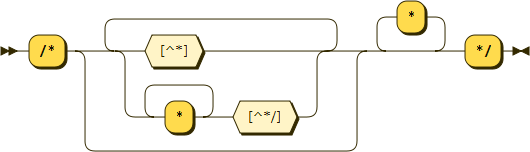
\includegraphics[scale=0.5]{kepek/rr_comment.png}
\caption{Comment}
\label{fig:rr_comment}
\end{figure}

\begin{figure}[h!]
\centering
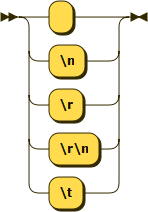
\includegraphics[scale=0.5]{kepek/rr_whitespace.png}
\caption{Whitespace}
\label{fig:rr_whitespace}
\end{figure}

\begin{figure}[h!]
\centering
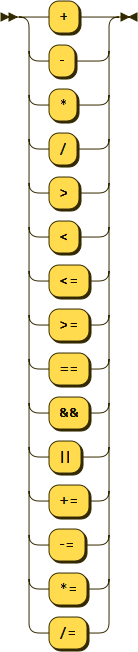
\includegraphics[scale=1]{kepek/rr_operator.png}
\caption{Operator}
\label{fig:rr_operator}
\end{figure}

\begin{figure}[h!]
\centering

\includegraphics[scale=1]{kepek/rr_digit.png}
\caption{Digit}
\label{fig:rr_digit}
\end{figure}

\begin{figure}[h!]
\centering
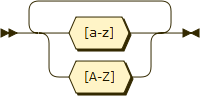
\includegraphics[scale=1]{kepek/rr_character.png}
\caption{Character}
\label{fig:rr_character}
\end{figure}

\begin{figure}[h!]
\centering
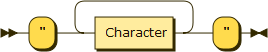
\includegraphics[scale=1]{kepek/rr_string.png}
\caption{String}
\label{fig:rr_string}
\end{figure}

\begin{figure}[h!]
\centering

\includegraphics[scale=1]{kepek/rr_block.png}
\caption{Block}
\label{fig:rr_block}
\end{figure}

\begin{figure}[h!]
\centering
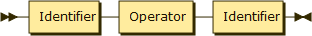
\includegraphics[scale=1]{kepek/rr_binaryoperator.png}
\caption{BinaryOperator}
\label{fig:rr_binaryoperator}
\end{figure}

\begin{figure}[h!]
\centering
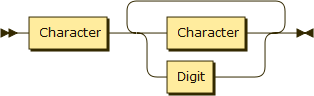
\includegraphics[scale=0.5]{kepek/rr_identifier.png}
\caption{Identifier}
\label{fig:rr_identifier}
\end{figure}

\begin{figure}[h!]
\centering
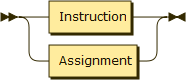
\includegraphics[scale=0.5]{kepek/rr_expression.png}
\caption{Expression}
\label{fig:rr_expression}
\end{figure}

\begin{figure}[h!]
\centering
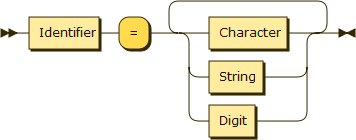
\includegraphics[scale=1]{kepek/rr_assignment.png}
\caption{Assignment}
\label{fig:rr_assignment}
\end{figure}

\begin{figure}[h!]
\centering
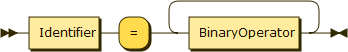
\includegraphics[scale=0.7]{kepek/rr_instruction.png}
\caption{Instruction}
\label{fig:rr_instruction}
\end{figure}

\begin{figure}[h!]
\centering
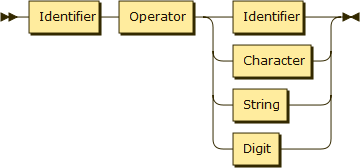
\includegraphics[scale=0.4]{kepek/rr_condition.png}
\caption{Condition}
\label{fig:rr_condition}
\end{figure}

\begin{figure}[h!]
\centering
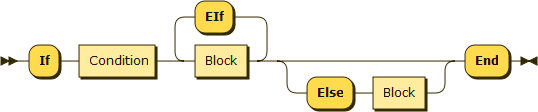
\includegraphics[scale=0.4]{kepek/rr_if.png}
\caption{If}
\label{fig:rr_if}
\end{figure}

\begin{figure}[h!]
\centering
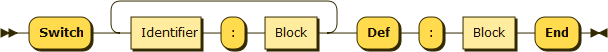
\includegraphics[scale=0.4]{kepek/rr_switch.png}
\caption{Switch}
\label{fig:rr_switch}
\end{figure}

\begin{figure}[h!]
\centering
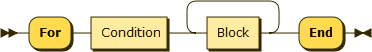
\includegraphics[scale=0.4]{kepek/rr_for.png}
\caption{For}
\label{fig:rr_for}
\end{figure}

\begin{figure}[h!]
\centering
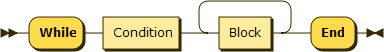
\includegraphics[scale=0.4]{kepek/rr_while.png}
\caption{While}
\label{fig:rr_while}
\end{figure}

\begin{figure}[h!]
\centering
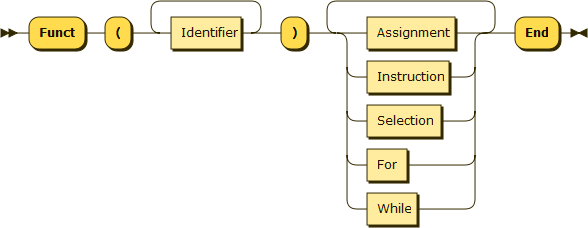
\includegraphics[scale=0.4]{kepek/rr_function.png}
\caption{Function}
\label{fig:rr_function}
\end{figure}

\begin{figure}[h!]
\centering
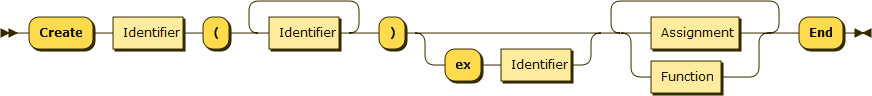
\includegraphics[scale=0.4]{kepek/rr_class.png}
\caption{Class}
\label{fig:rr_class}
\end{figure}

\begin{figure}[h!]
\centering

\includegraphics[scale=1]{kepek/rr_program.png}
\caption{Program}
\label{fig:rr_program}
\end{figure}

\section{Példák}

Egy példa forráskód részlet, melyben egy osztály és a benne lévő elemek láthatók

\begin{verbatim}
Create Ember
	
	Ember(string nev, int kor, int irSzam, string utca, int hSz)
		string @nev = nev
		int @kor = kor
		Cim @cim = Cim(irSzam, utca, hSz)
	End
		
	Funct void @decrKor(int szam)
		While szam>0
			@kor = @kor - 1
			@szam = @szam --
		End
	End
	
	Funct string @createString()
		@nev + @kor + @cim.createString
	End
End
\end{verbatim}
		
Az alábbiakban a fenti osztály példányosítása és használatának példája látható

\begin{verbatim}
Ember pelda = Ember("teszt", 20, 1542, "Teszteles", 50)
pelda.setParam1("TesztKetto")
string ember = pelda.createString
\end{verbatim}
